\section{Einleitung}

\begin{frame}
  \begin{itemize}
  \item Ziel: Leitfähigkeiten der Ionenkanäle ermitteln
  \item Basis Bachelorarbeit von Anne Kloskowki
  \item Erreicht:
    \begin{itemize}
    \item alternative Variatoren, Selektoren und Replacer
    \item GUI
    \item schnellerer Code ($>3\times$ speedup); Nebenläufigkeit von Konfigurationen
    \item persistente Ausgabe (Datei, Zeitstempel)
    \end{itemize}
  \end{itemize}
\end{frame}


\subsection{Neuronenmodelle}

\begin{frame}
  \begin{itemize}
    % Novak et al.
  \item 4 Neuronenklassen
    \begin{itemize}
    \item regular spiking
    \item fast spiking
    \item intrinsic bursting
    \item chattering
    \end{itemize}
  \end{itemize}
\end{frame}




\section{Genetischer Algorithmus}

\subsection{Einleitung}

\begin{frame}
  \frametitle{Genetischer Algorithmus}
  \begin{columns}[T]
    \begin{column}{0.35\textwidth}
      \begin{itemize}
      \item Idee: biologische Evolution
      \item effizient bei komplexen Fitness Beziehungen
      \item Überwindung lokaler Maxima
      \end{itemize}
    \end{column}
    \begin{column}{0.65\textwidth}
        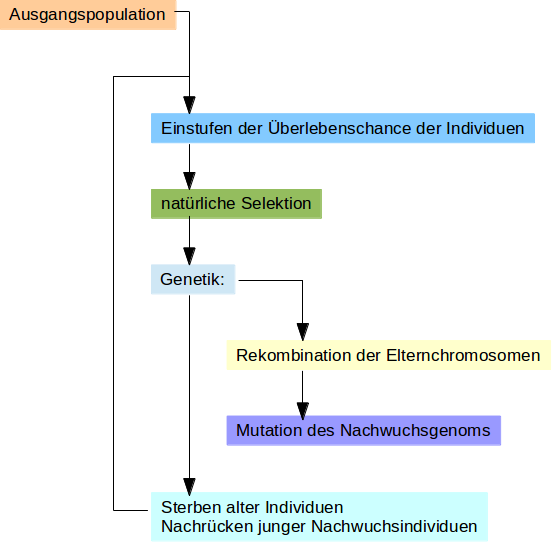
\includegraphics[width=\textwidth]{GenAlg-Diagramm.png}
        \captionsource{\tiny Evolutionäre Algorithmen zur Parametereinstellung
          in elektrophysiologischen Neuronenmodellen, Anne Kloskowski, 2013}
    \end{column}
  \end{columns}
\end{frame}


\subsection{GUI}

\begin{frame}
  \frametitle{GUI}
  \begin{block}{Features}
    \begin{itemize}
    \item Speichern/Laden von Konfigurationen
    \item Auswahl des Algorithmus'
    \item Einstellung der Parameter
    \end{itemize}
  \end{block}
  \only<2->{
    \center
    \LARGE
    Anwendungsbeispiel
  }
\end{frame}

\subsection{Ergebnisse}

\begin{frame}
  \frametitle{Durchführung}
  \begin{itemize}
  \item 44 Simulationen
  \item eine Baseline je Neuronklasse
    \scriptsize
    \begin{tabular}[H]{ll}
      Parameter & Werte \\\hline
      Populationsgröße & 50, 125, 200 \\ \arrayrulecolor{light-gray}\hline
      Tournament Selection, Tournamentgröße & 5, 15 \\
      Fitness Proportionate Selection & \\
      Truncation Selection  & \\ \hline
      Mutationsstärke & 0.08333, 0.15, 0.25 \\ \hline
      Random Replacement, elites & 0, 5, 10 \\
      Truncation Replacement & \\
    \end{tabular}
  \end{itemize}
\end{frame}


% RS: mut-strength(alle)
% IB: popsize(alle)
% FS: alle selections, 4 Stück
% CH: 
\begin{frame}
  
\end{frame}

\subsection{Aussicht}

\begin{frame}
  \begin{itemize}
  \item Kombination von zielführenden Parametern
  \item Anpassung der Fitnessfunktion
  \item mehrfache Ausführung der Läufe
  \end{itemize}
\end{frame}